\section{Simulación de la señal de SUSY}\label{sec:sig_samples}

Como se ha mencionado en el \cref{cap:susy}, debido al gran número de parámetros
libres en los modelos de SUSY, las búsquedas de supersimetría en ATLAS están
impulsadas por la fenomenología de los estados finales. El análisis realizado
para esta tesis está motivado por estados finales con fotones energéticos,
provenientes del decaimiento de un neutralino NLSP en el contexto de modelos
GGM.

En los modelos GGM el decaimiento de los estados supersimétricos producidos en
las colisiones del LHC van a proceder por medio de decaimientos en cascada hasta
el neutralino NLSP que decaerá a un gravitino y una partícula del SM, que
dependerá de la naturaleza de la NSLP. Distintas posibilidades para la
naturaleza de la NLSP pueden ser consideradas, las cuales dan lugar a estados
finales distintos y complementarios entre si, para cubrir las distintas regiones
del espacio de fase de los modelos GGM. Dentro de ATLAS se exploraron cuatro
estados finales diferentes: dos fotones, un fotón y un leptón, un fotón y
{\bjets}, y un fotón y jets, todos con energía faltante, correspondiente a los
gravitinos LSP.

En particular en esta tesis se focalizó en el análisis de un estado final que
consiste en un único fotón, jets y energía faltante.
La selección de eventos que se describe en el \cref{cap:seleccion} fue diseñada para
maximizar la sensibilidad a pequeñas señales con esta topología general.
Cualquier imposición de cortes muy dependientes del modelo fueron evitadas,
tratando de mantener el análisis lo más independiente del modelo como fuera
posible. Sin embargo, una interpretación en el marco de un modelo especifico es
inevitable. Con tal motivo se simuló un conjunto de puntos de señal con
distintos valores de los parámetros para cubrir la región del espacio de
parámetros donde pueda manifestarse dicha señal.

%% Se simularon puntos de senal para la produccion de gluinosLos resultados se interpretaron
%% son interpretados en el contexto de GGM que
%% incluyen la produccion de supercompaneras de particulas del SM que se acoplan
%% fuertemente comot ambien de que poseen solo carga electrodebil.

Se utilizó un espectro simplificado en el cual, básicamente, el espacio de
parámetros consiste en la escala de producción (por simplicidad, la masa del
gluino) y la masa de la NLSP. Todos los demás estados fueron desacoplados ya que
no juegan un rol importante en la producción o en el estado final de interés.
Esta aproximación es similar a los denominados <<modelos simplificados>>
utilizados en otras búsquedas.
La masa del gluino es el único parámetro libre de las partículas de color para
poder determinar un límite conservativo en la masa del mismo. Todos los
parámetros de masa \emph{soft} de los \emph{squarks} se fijan en 2.5 \tev.

Para maximizar la probabilidad de tener un único fotón en el estado final, es
necesario que $\mathrm{BR}(\ninoone \to \gam\,\gravino) \sim 50\%$. Esto resulta
cuando el neutralino más liviano es una mezcla bino-higgsino. Además, el valor
de $\mu$ debe ser positivo para suprimir el decaimiento a Higgs, que llevará a
un estado final ya cubierto por otro análisis de ATLAS. Para lograr la BR
deseada se variaron los parámetros de masa de bino ($M_1$) y higgsinos ($\mu$)
para las diferentes masas del {\ninoone}, de tal forma que los BR del {\ninoone}
sean aproximadamente constantes:

\begin{align}
  &\mathrm{BR}(\ninoone \to \gam\, \gravino) \approx 50\% \label{eq:n1_gam}\\
  &\mathrm{BR}(\ninoone \to Z\, \gravino) \approx 49\%    \label{eq:n1_z} \\
  &\mathrm{BR}(\ninoone \to h\, \gravino) \approx 1\%     \label{eq:n1_h}
\end{align}


Los demás parámetros del modelo se fijan en $M_2=2.5\tev$, $\tan\beta=1.5$ y
$c\tau_{\mathrm{NLSP}} < 0.1$ mm. Este último asegura que el neutralino decaiga
rápidamente dentro del detector y se logra haciendo al gravitino lo
suficientemente liviano ($m_{\tilde{G}}=10^{-9} \gev$). Todos los términos
tri-lineares son fijados a cero y las masas de los sleptones a $2.5 \tev$.
Las masas del higgs liviano ($h$) y el pseudoescalar ($A$) se fijan a
$m_{h} = 126 \gev$ y $m_{A} = 2 \tev$.
La masa del $h$ se considera a partir del valor
medido de la masa del Higgs observado en el a\~no 2012.
En modelos GGM de SUSY existen distintos
mecanismos\cite{Craig:2011yk,Auzzi:2011eu,Csaki:2012fh,Larsen:2012rq,Craig:2012hc}
para generar una masa del bosón de Higgs tan alta como este valor observado, sin
cambiar la fenomenología de los modelos considerados. No se observó un efecto
significativo en el espectro de masas variando el valor de la masa de Higgs en un
rango de $\pm 10 \gev$.
%% Tambien se estudio el efecto de variar el valor
%% de $\tan\beta$\note{Hacer comentario de $\tan\beta$}

A partir de estos estudios se procedió a simular un conjunto de puntos de señal
(\emph{grid}) en el plano ($m_{\gluino}$, $m_{\ninoone}$), variando los parámetros
$M_3$ y $\mu$. El parámetro $M_1$ se ajustó, dependiendo del $\mu$ de forma de
obtener las BR descriptas anteriormente. La \emph{grid} cubre el espacio $150\gev <
m_{\ninoone} < 1250 \gev$ y $800\gev < m_{\gluino} < 1300 \gev$, con
$m_{\ninoone} < m_{\gluino}$ (ver \cref{fig:gridpoints}).


\begin{figure}[!htb]
  \centering
  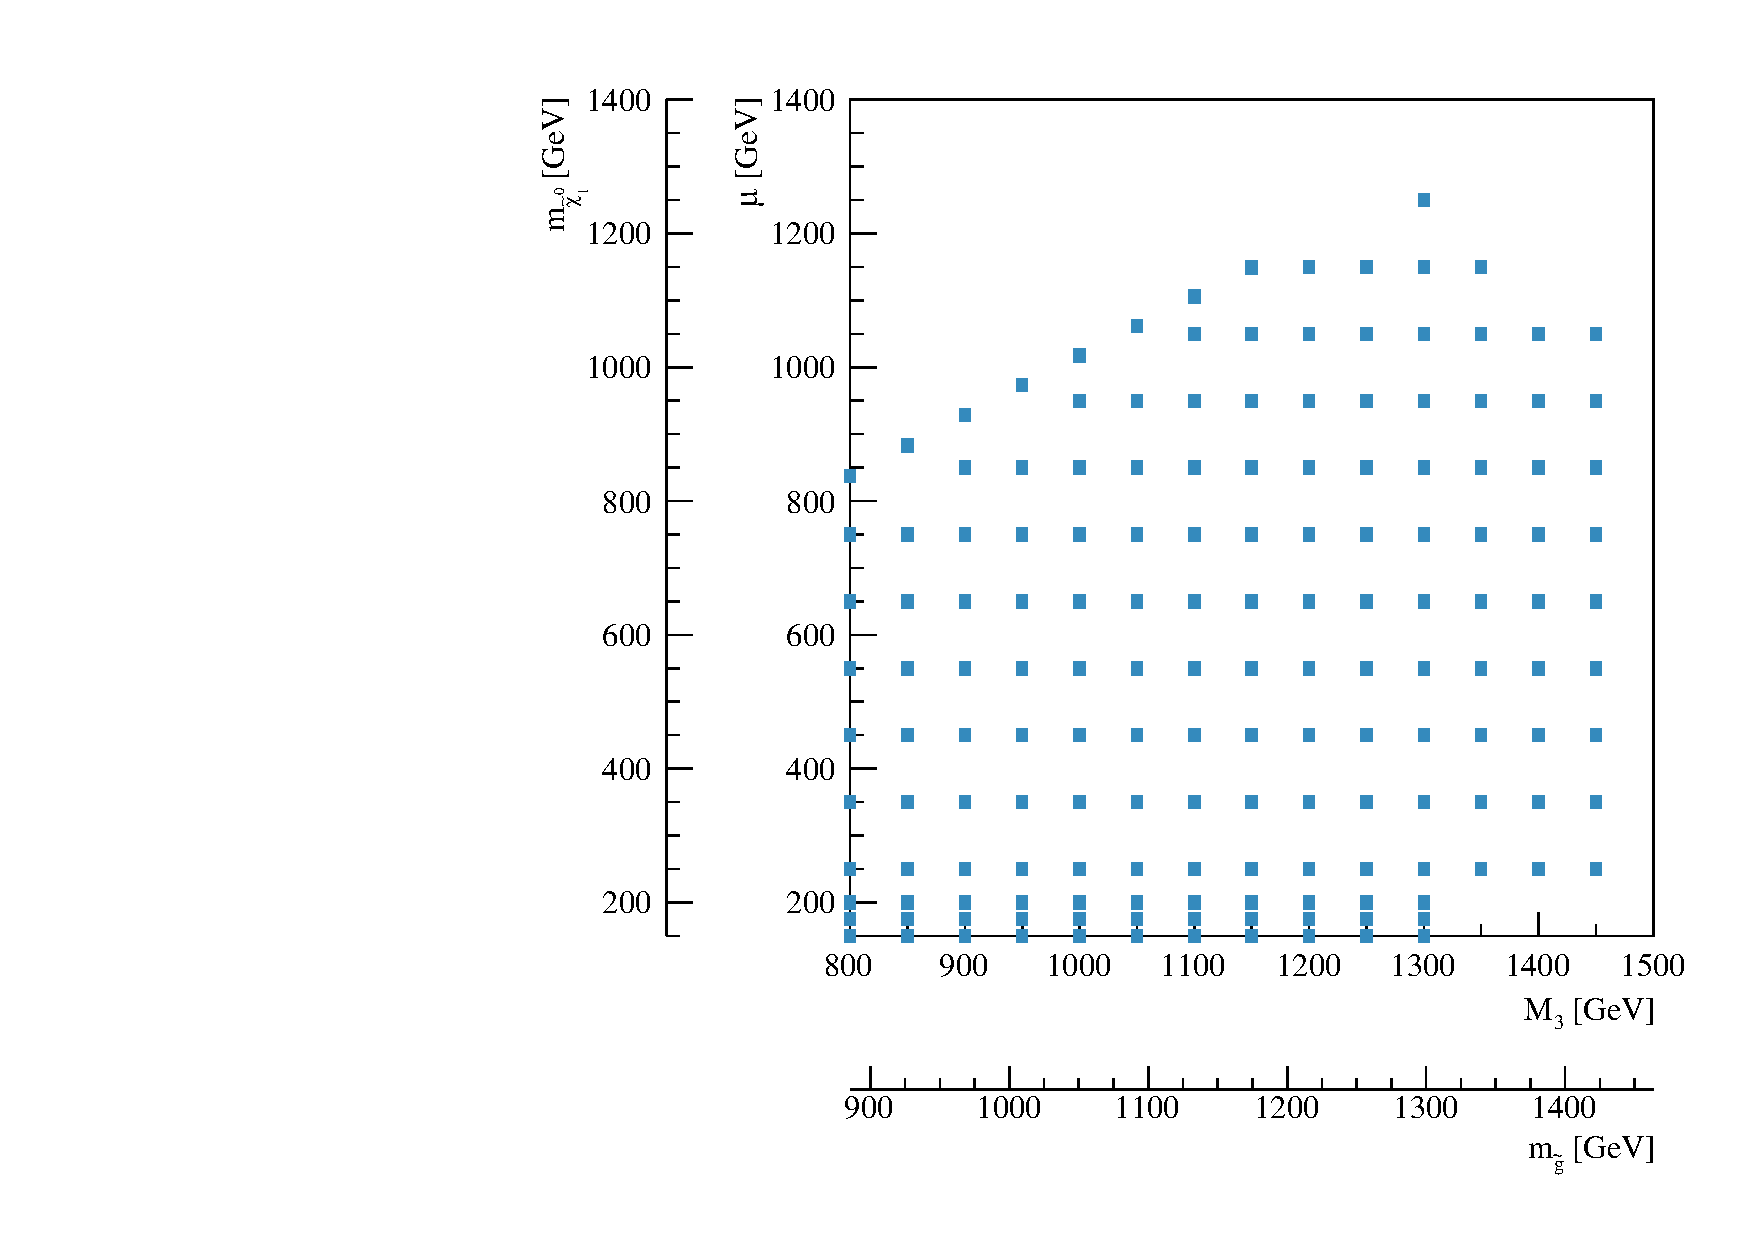
\includegraphics[width=0.8\textwidth]{figures/run1_grid}
  \caption{Conjunto de puntos (\emph{grid}) de señal simulada para el presente
    análisis. Los cuadrados azules representan los distintos puntos de señal
    generados con distintos valores de $m_{\gluino}$ y $m_{\ninoone}$. También
    puede verse la relación con las masas $m_{\gluino}$ y $m_{\ninoone}$.}
  \label{fig:gridpoints}
\end{figure}


El espectro completo de masas y los correspondientes decaimientos fueron
calculados a partir de estos parámetros utilizando {\suspect}
(v2.41)\cite{Djouadi2007426}, {\sdecay} (v1.3b)\cite{Muhlleitner:2004mka} y
{\hdecay} (v3.4)\cite{Djouadi:1997yw}, que forman parte del paquete {\susyhit}
(v1.3)\cite{Djouadi:2006bz}. Algunos ejemplos del espectro de masas pueden verse
en la \cref{fig:mass_spectra}, para algunos puntos de la \emph{grid}, (885, 146) y (1463, 1053).

\begin{figure}[!htb]
   \centering
   \includegraphics[width=0.45\textwidth]{figures/masses_GGM_M3_mu_800_150}
   %%\includegraphics[width=0.45\textwidth]{figures/masses_GGM_M3_mu_1000_750}
   \includegraphics[width=0.45\textwidth]{figures/masses_GGM_M3_mu_1450_1050}

   \caption{Espectro de masas de las partículas supersimétricas para dos puntos de la \emph{grid} de señal.
     En la izquierda para (885,146) y en la derecha (1463, 1053), en el plano \mgmn.}
     %% Solo $M_3$ y $\mu$ son los parámetros libres, en este caso
     %% $(M_3, \mu) = (800~\gev, 250~\gev)$. }
   \label{fig:mass_spectra}
\end{figure}

Para cada uno de los 124 puntos de señal que constituyen la \emph{grid} se generaron
5000 eventos, utilizando {\herwigpp} v2.5.2\cite{Bahr:2008pv} y el conjunto de
PDFs CTEQ6L1\cite{Nadolsky:2008zw}. Se aplicó un filtro a nivel generador, que
requería la presencia de un fotón con un {\pt} de al menos 100 \gev, para
optimizar la generación, especialmente en los puntos donde el
neutralino tiene menor masa. La eficiencia del filtro para todas las muestras
simuladas puede verse en la \cref{tab:signal_filter_eff}. La simulación del
detector ATLAS se realizó con la simulación rápida
\textsc{ATLFAST-II}\cite{Richter-Was:683751}.


\begin{table}[!htb]
  \centering
  \caption{Relación entre los parámetros libres del modelo $M_3$ y $\mu$ con las
    masas $m_{\gluino}$ (izquierda) y $m_{\ninoone}$ (derecha), respectivamente.
    En la tabla de la derecha, para cada valor de $\mu$ también se puede
    observar el valor de $M_1$ utilizado para obtener los BR de decaimiento del
    {\ninoone} deseados.}
  \label{tab:signal_pars}

  \begin{minipage}[!t]{0.5\textwidth}
    \centering
    \begin{tabular}{cc}
      \hline
      $M_3$ [\gev]& $m_{\gluino}$ [\gev] \\
      \hline
      800  & 885.5 \\
      850  & 931.7 \\
      900  & 977.6 \\
      950  & 1023.1 \\
      1000 & 1068.3  \\
      1050 & 1113.3  \\
      1100 & 1157.9  \\
      1150 & 1202.3  \\
      1200 & 1246.4  \\
      1250 & 1290.3  \\
      1300 & 1333.9  \\
      1350 & 1377.3  \\
      1400 & 1420.5  \\
      1450 & 1463.4  \\
      \hline
    \end{tabular}
    \vspace{5cm}
  \end{minipage}%
  \begin{minipage}[t]{0.5\textwidth}
    \begin{tabular}{ccc}
      \hline
      $\mu$ [\gev] & $M_1$ [\gev] & $m_{\ninoone}$ [\gev] \\
      \hline
      150  &  300  & 147.0 \\
      175  &  270  & 168.3 \\
      200  &  267  & 190.3 \\
      250  &  288  & 235.8 \\
      350  &  365  & 332.4 \\
      450  &  456  & 433.2 \\
      550  &  551  & 535.6 \\
      650  &  647  & 638.3 \\
      750  &  745  & 742.0 \\
      838  &  837  & 836.4 \\
      850  &  845  & 846.7 \\
      883  &  882  & 883.7 \\
      928  &  926  & 930.2 \\
      950  &  942  & 949.6 \\
      973  &  970  & 976.6  \\
      1017 &  1015 & 1023.4 \\
      1050 &  1040 & 1053.0 \\
      1062 &  1058 & 1068.9 \\
      1106 &  1102 & 1114.8 \\
      1149 &  1145 & 1160.0 \\
      1150 &  1140 & 1157.5 \\
      1250 &  1238 & 1260.6 \\
      \hline
    \end{tabular}

  \end{minipage}

\end{table}


\begin{table}[ht]
  \centering

  \footnotesize
  \caption{Eficiencia del filtro a nivel generador [\%]
    para los puntos de señal simulados.}
  \begin{tabular}{c|ccccccccccccccccc}
    \hline
     &   \multicolumn{14}{c}{ $M_3$ [\gev] } \\
    $\mu$ [\gev] &  800 & 850 & 900 & 950 & 1000 & 1050 & 1100 &1150 & 1200  & 1250 & 1300 & 1350 & 1400 & 1450 \\
    \hline
    150  &   39.54 &   39.8 &  41.9    &   42.6   &   43.0   &   44.2   &   45.5    &   46.3    &    47.1  &   48.3  &   49.1 &      &      &       \\
    175  &   44.55 &   44.6 &  46.5    &   47.5   &   47.8   &   48.9   &   50.3    &   51.4    &    51.5  &   52.4  &   53.3 &      &      &       \\
    200  &   47.66 &   48.4 &  50.1    &   50.6   &   52.0   &   52.8   &   53.8    &   55.0    &    55.0  &   56.2  &   56.0 &      &      &       \\
    250  &   55.09 &   56.0 &  56.1    &   57.1   &   56.7   &   58.0   &   58.9    &   59.5    &    60.5  &   60.7  &   61.2 & 62.1 & 62.2 &  63.9 \\
    350  &   65.82 &   66.1 &  64.6    &   65.8   &   66.4   &   66.7   &   66.5    &   67.7    &    67.4  &   67.6  &   67.8 & 68.0 & 69.2 &  68.4 \\
    450  &   71.29 &   71.4 &  71.4    &   71.8   &   72.1   &   72.5   &   72.0    &   72.6    &    72.1  &   72.5  &   73.4 & 72.9 & 72.2 &  73.4 \\
    550  &   73.08 &   72.5 &  73.3    &   73.7   &   74.6   &   74.3   &   75.0    &   74.8    &    74.2  &   74.7  &   75.6 & 75.7 & 74.9 &  75.3 \\
    650  &   69.78 &   72.0 &  73.2    &   74.1   &   75.6   &   76.2   &   75.9    &   75.8    &    77.0  &   77.0  &   76.2 & 76.7 & 77.1 &  76.6 \\
    750  &   47.69 &   60.2 &  66.9    &   70.4   &   73.4   &   74.0   &   75.9    &   76.5    &    77.1  &   77.3  &   76.3 & 77.9 & 77.2 &  77.0 \\
    838  &    9.0  &        &          &          &          &          &           &           &          &         &        &      &      &       \\
    883  &         &   9.1  &          &          &          &          &           &           &          &         &        &      &      &       \\
    850  &         &        &  34.2    &   50.7   &   60.1   &   66.4   &   70.4    &   73.5    &    73.6  &   75.4  &   76.6 & 77.1 & 78.2 &  76.8 \\
    928  &         &        &   9.4    &          &          &          &           &           &          &         &        &      &      &       \\
    950  &         &        &          &          &   25.4   &   41.4   &   54.0    &   62.2    &    66.8  &   70.9  &   75.2 & 75.9 & 78.1 &  77.2 \\
    973  &         &        &          &   10.0   &          &          &           &           &          &         &        &      &      &       \\
    1017 &         &        &          &          &   10.3   &          &           &           &          &         &        &      &      &       \\
    1050 &         &        &          &          &          &          &   19.2    &   31.6    &    45.2  &   56.8  &   62.7 & 68.9 & 73.1 &  75.6 \\
    1062 &         &        &          &          &          &   11.1   &           &           &          &         &        &      &      &       \\
    1106 &         &        &          &          &          &          &   11.7    &           &          &         &        &      &      &       \\
    1149 &         &        &          &          &          &          &           &   12.6    &          &         &        &      &      &       \\
    1150 &         &        &          &          &          &          &           &           &    16.1  &   24.9  &   36.9 & 49.0 &      &       \\
    1250 &         &        &          &          &          &          &           &           &          &         &   16.1 &      &      &       \\
    \hline
  \end{tabular}
  \label{tab:signal_filter_eff}
\end{table}



\subsection{Estudios a nivel generador}
\label{sec:susy_studies}

Se realizaron algunos estudios para entender mejor el estado final y poder
identificar las distintas regiones en el espacio de fase, lo cual facilitaría el
proceso de optimización de las posibles regiones de se\~nal. En la
\cref{fig:signal_br_gl} se presentan los distintos BR de los gluinos para todos
los puntos de la \emph{grid}. Resulta evidente que la cadena de decaimiento dominante
varía en las distintas regiones de la \emph{grid}, dependiendo de la masa del gluino y
el neutralino. Se puede ver que el decaimiento dominante es a través de
charginos, pero a medida que la masa del gluino y el neutralino se acercan,
empieza a resultar más importante el decaimiento directo al neutralino más
liviano, mientras que en los puntos más cercanos a la diagonal, el decaimiento
estará dominado por $\gluino\to g\gravino$ el cual no corresponde al estado
final deseado. Los diagramas de los distintos decaimientos posibles se encuentran
en la \cref{fig:signal_diagrams}, de los cuales se pueden extraer varias
conclusiones: en el caso de las cadenas largas a través de charginos, el estado
final tendrá una mayor cantidad de jets. Si el decaimiento es directamente al
{\ninoone} la multiplicidad de jets será menor y la energía del fotón será mayor
al igual que la energía faltante.


\begin{figure}[!htb]
  \centering

  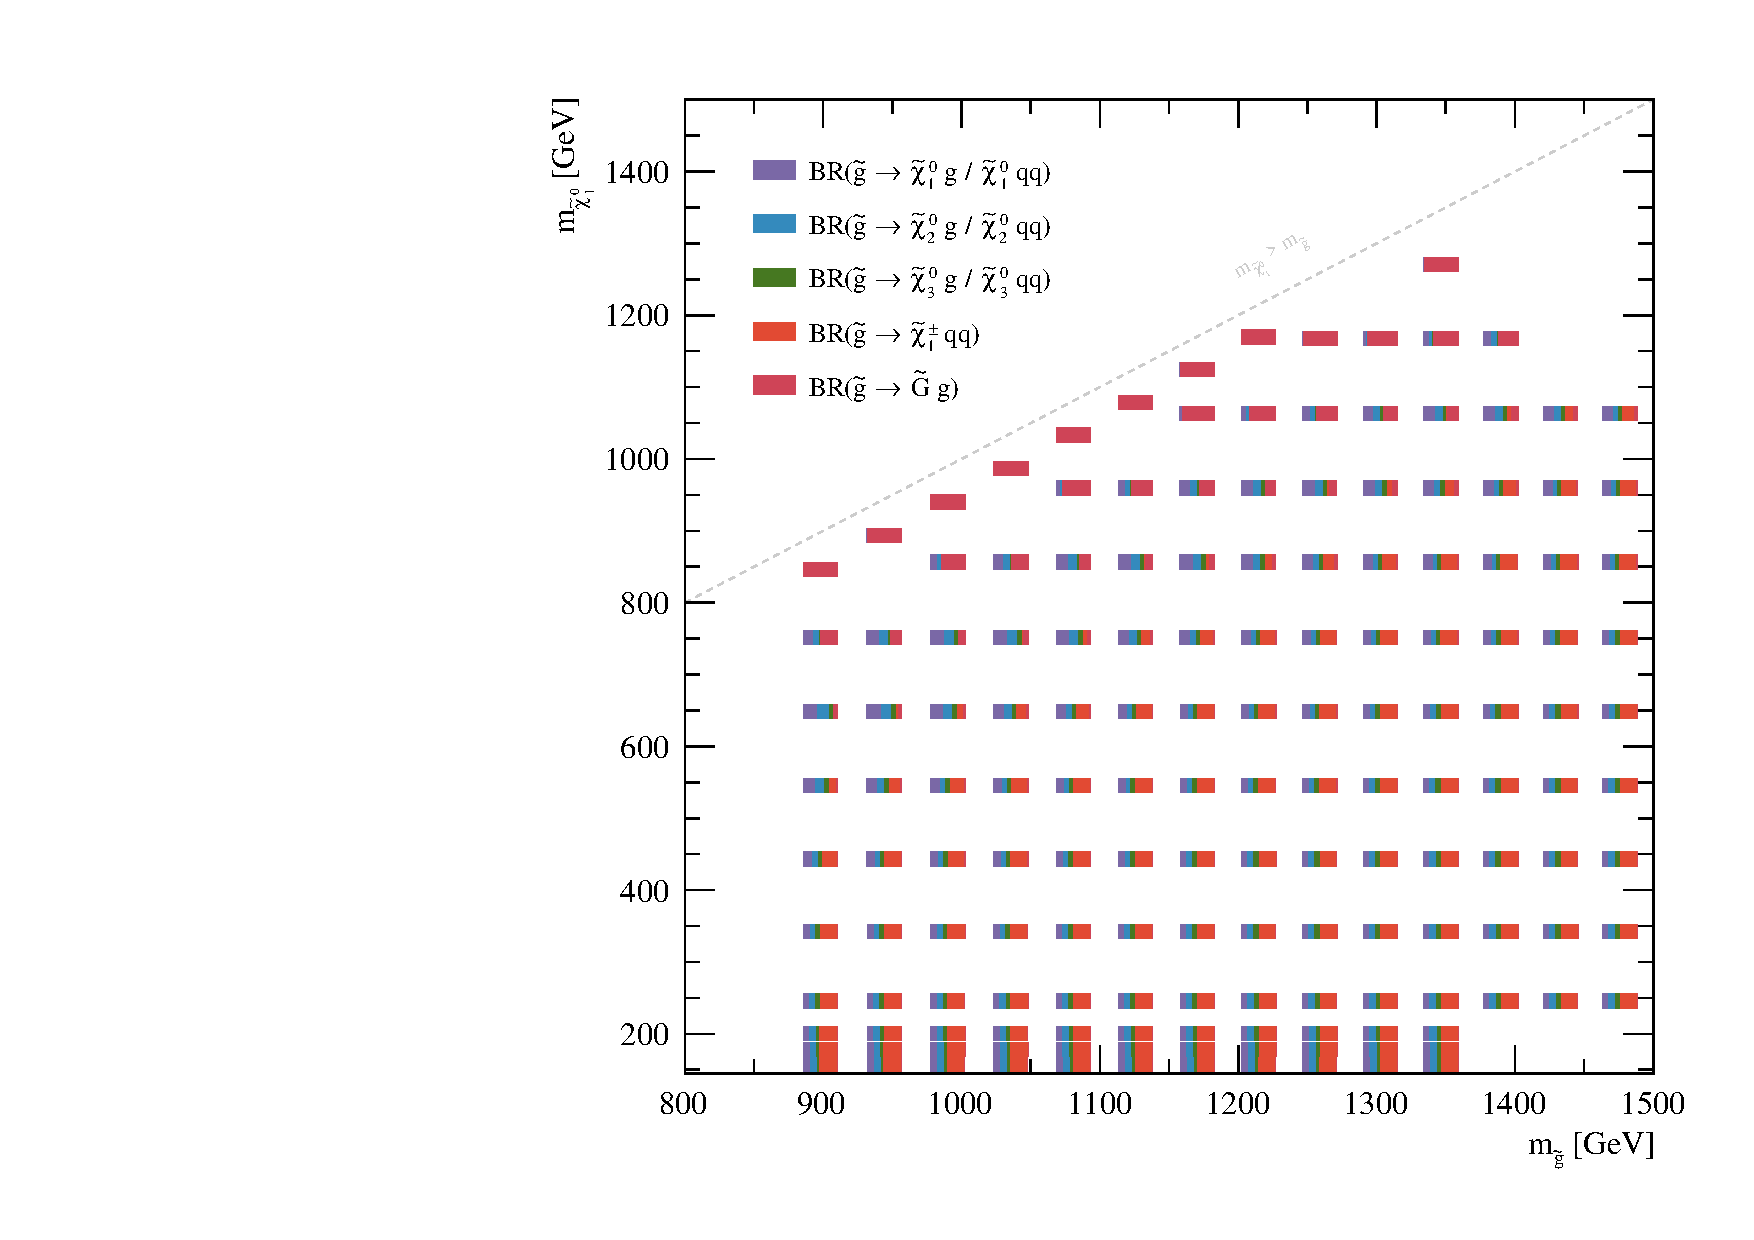
\includegraphics[width=0.6\textwidth]{figures/br_gl_X}

  \caption{Tasas de decaimiento (BR) de los gluinos para los distintos puntos de la \emph{grid} en
    el plano \mgmn. Para cada punto de señal, la fracción del rectángulo de cada color representa
    el BR a cada uno de los posibles estados finales.}
  \label{fig:signal_br_gl}
\end{figure}


\begin{figure}[!htb]
  \centering

  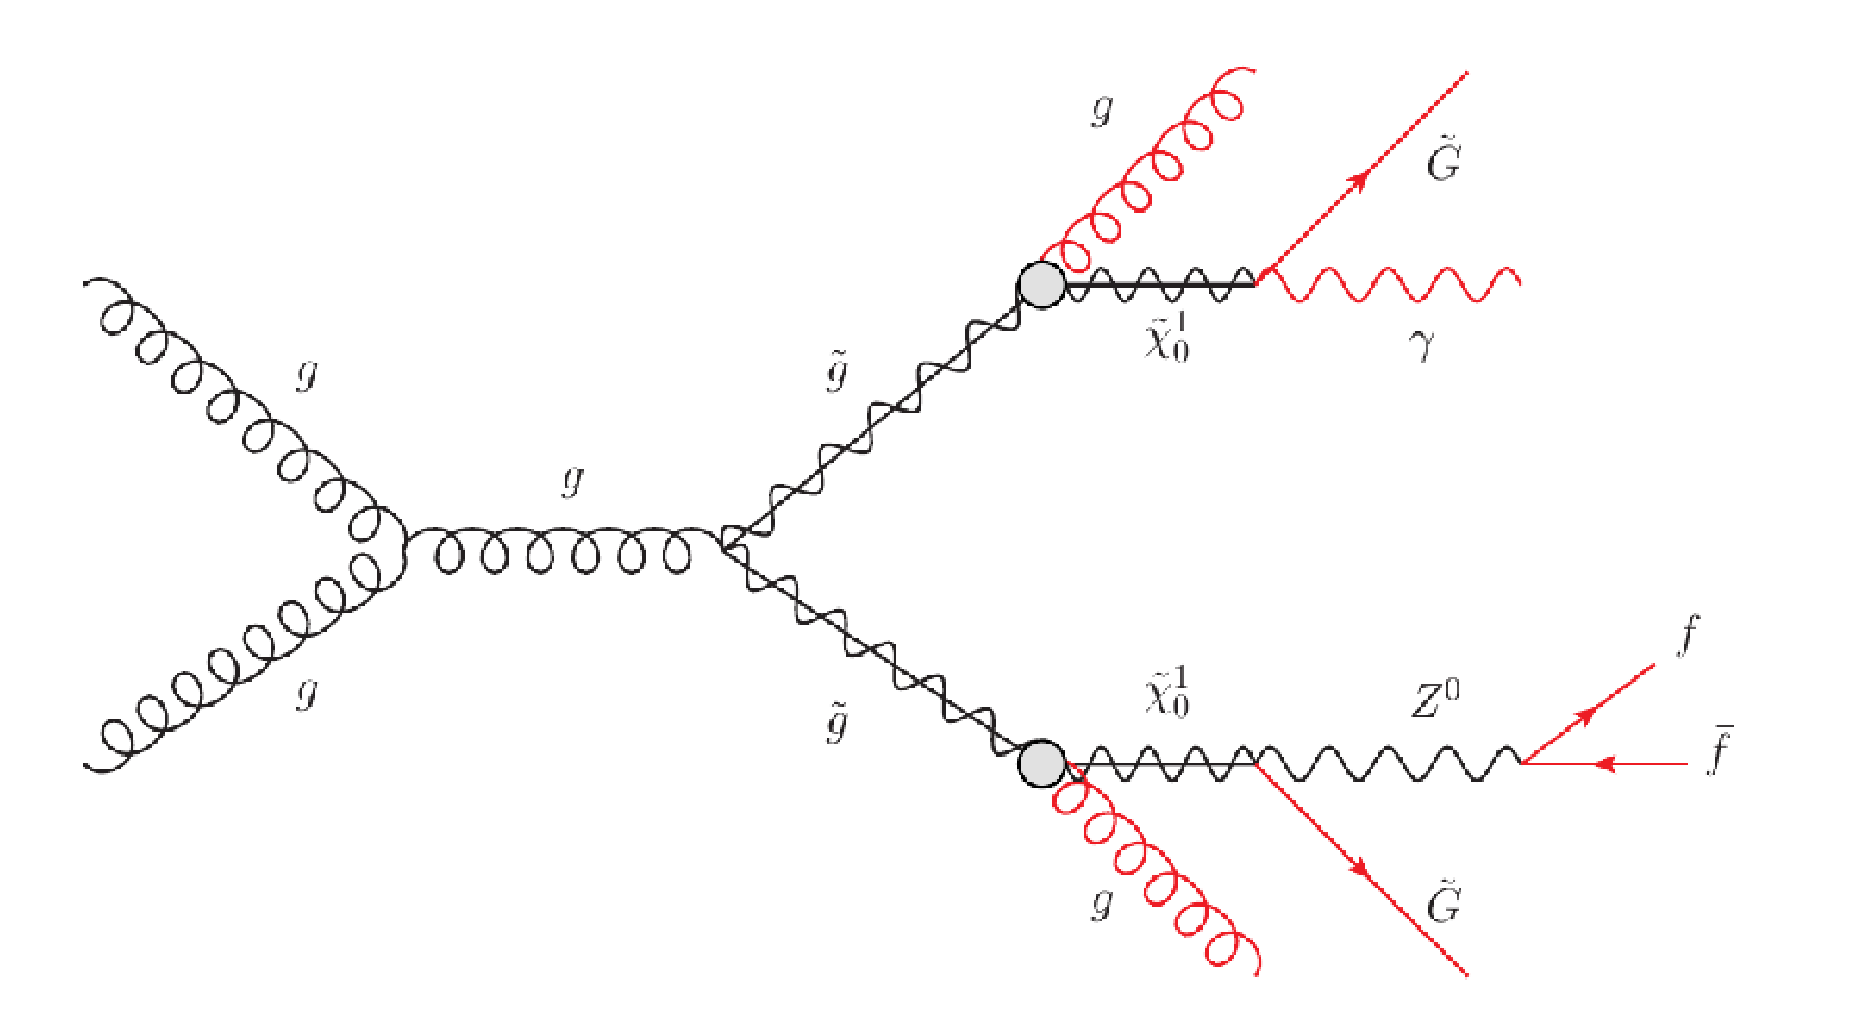
\includegraphics[width=0.49\textwidth]{diagram_a}
  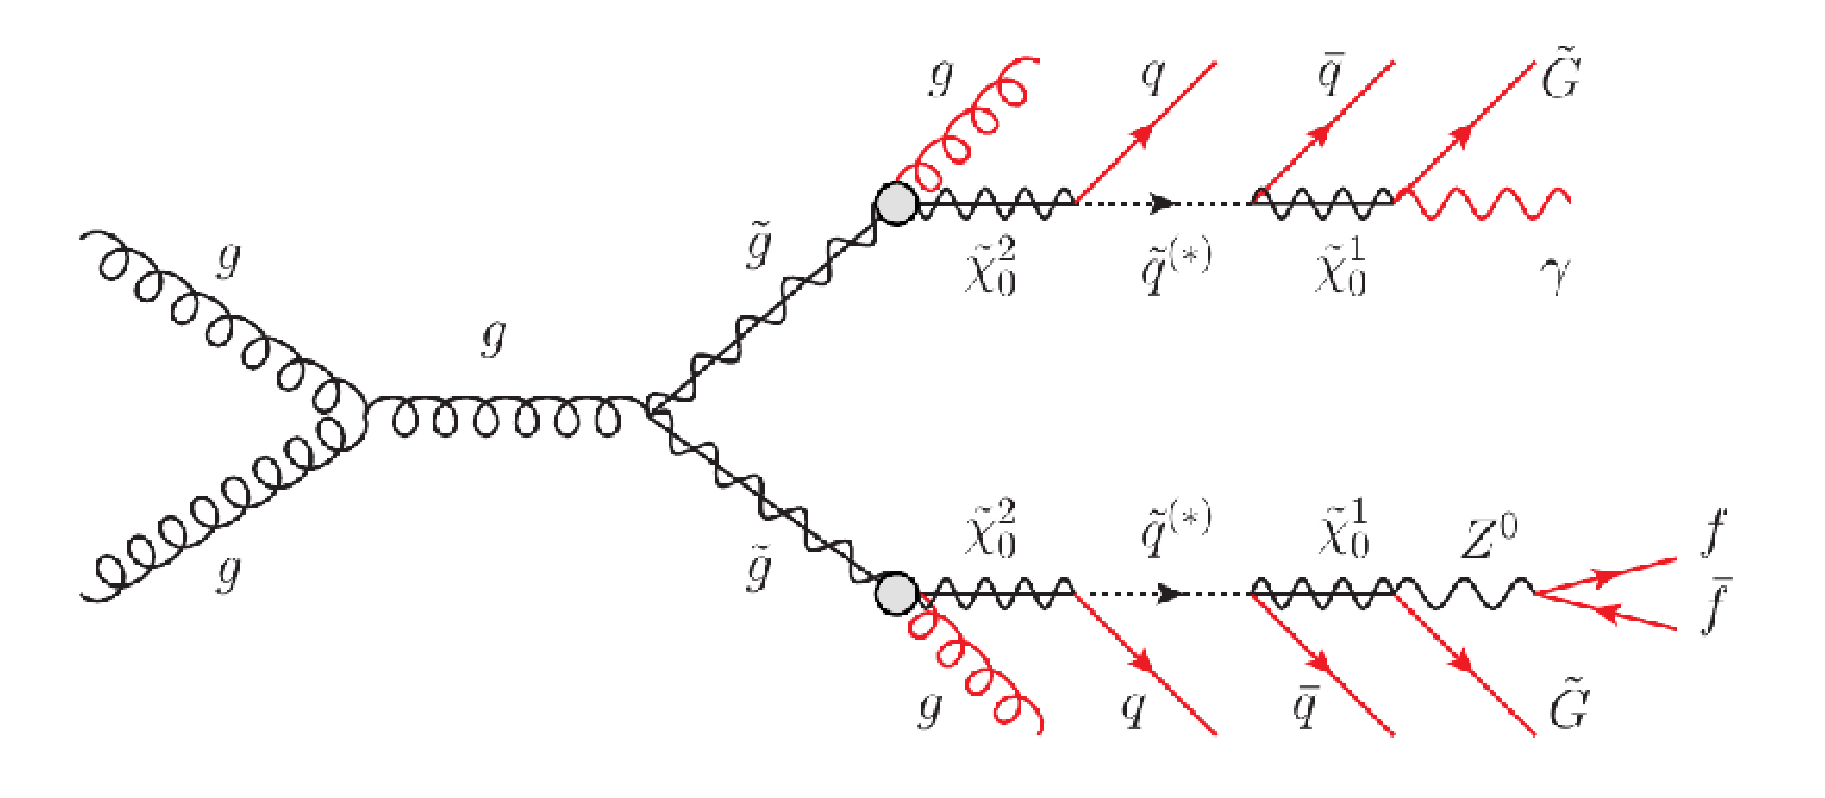
\includegraphics[width=0.49\textwidth]{diagram_b}

  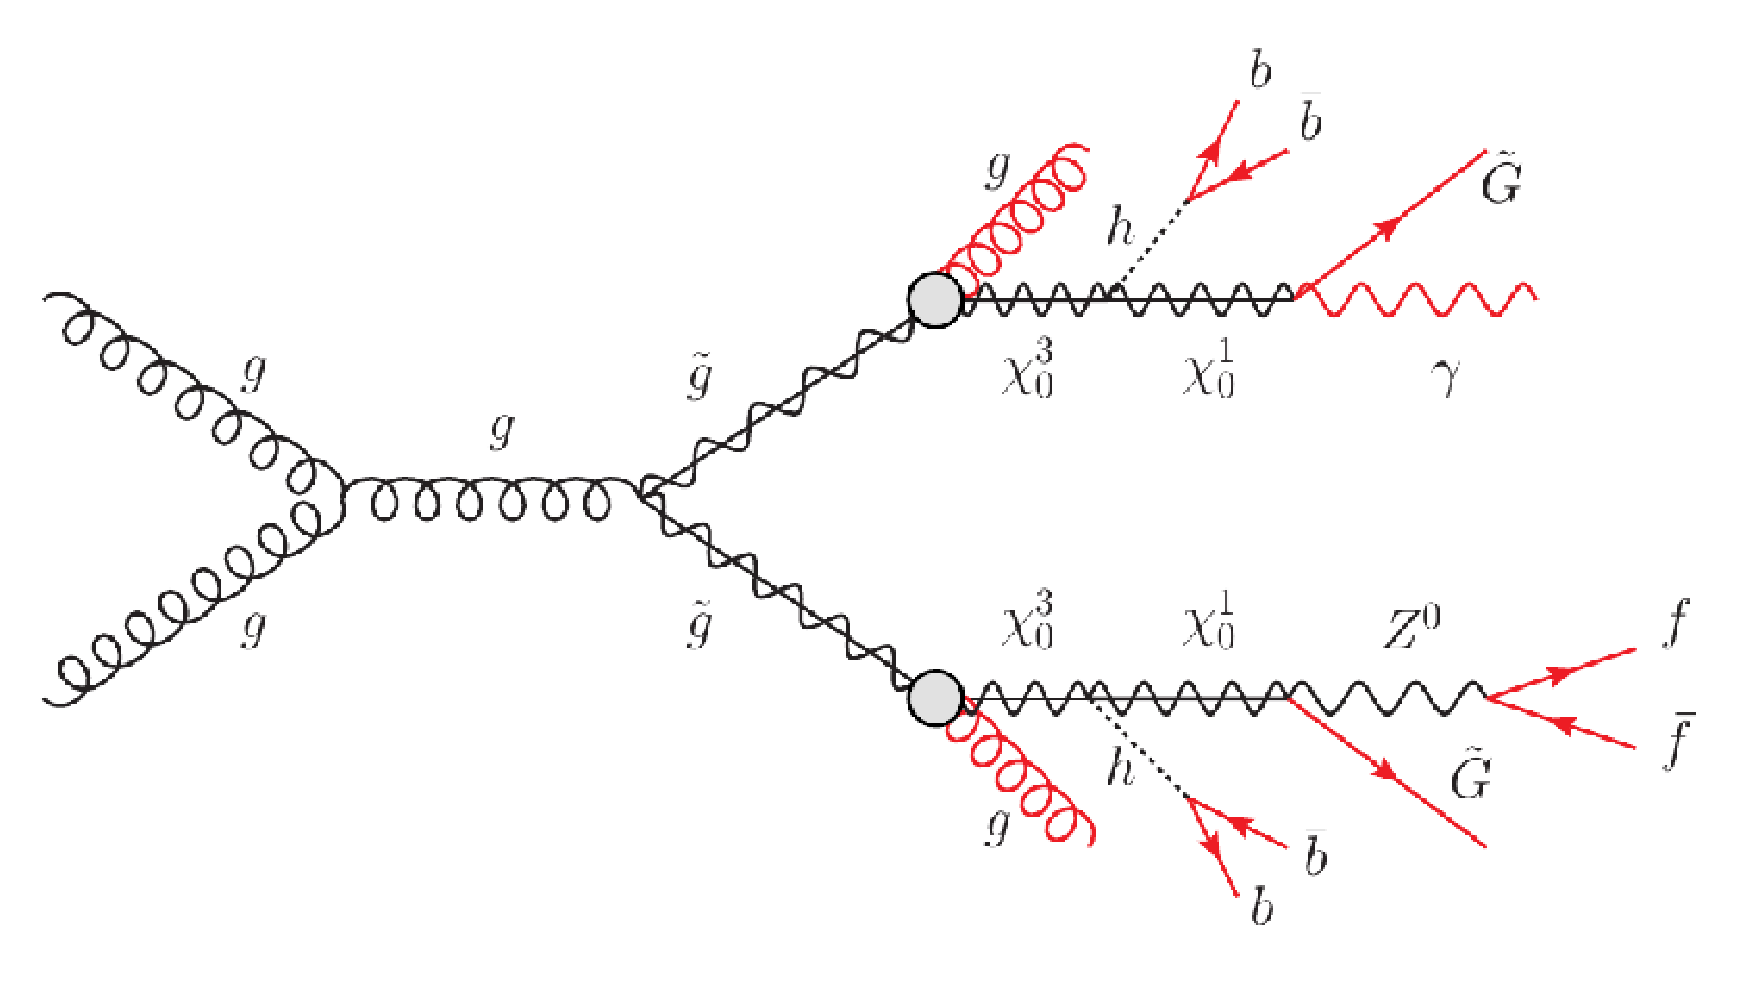
\includegraphics[width=0.49\textwidth]{diagram_c}
  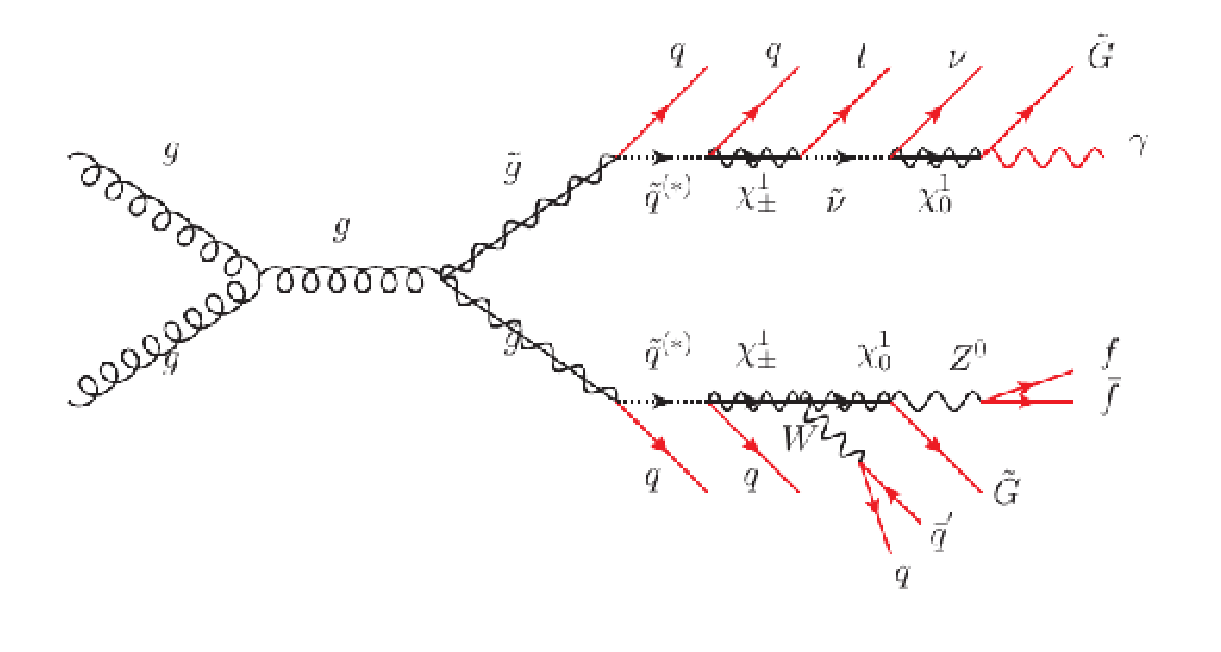
\includegraphics[width=0.49\textwidth]{diagram_d}

  \caption{Diagramas de Feynman para la producción de gluinos y el subsiguiente
    decaimiento de los mismos hasta el estado final. Los distintos diagramas ilustran ... }
  \label{fig:signal_diagrams}

\end{figure}


En la \cref{fig:signal_br_n1} se presentan las BR de decaimiento del neutralino
mas liviano (\ninoone), compatibles con las esperadas a partir del modelo que se
utilizará para el presente análisis (\cref{eq:n1_gam,eq:n1_z,eq:n1_h}). Estos
valores varían en menos del 1\% en los distintos puntos de la grid, salvo para
neutralinos livianos ($<200\gev$) donde la producción de Higgs es altamente
suprimida, mientras aumenta el decaimiento a $Z$, y $\mathrm{BR}(\ninoone \to
\gam \gravino)$ empieza a caer llegando al 40\%.

\begin{figure}[!htb]
  \centering

  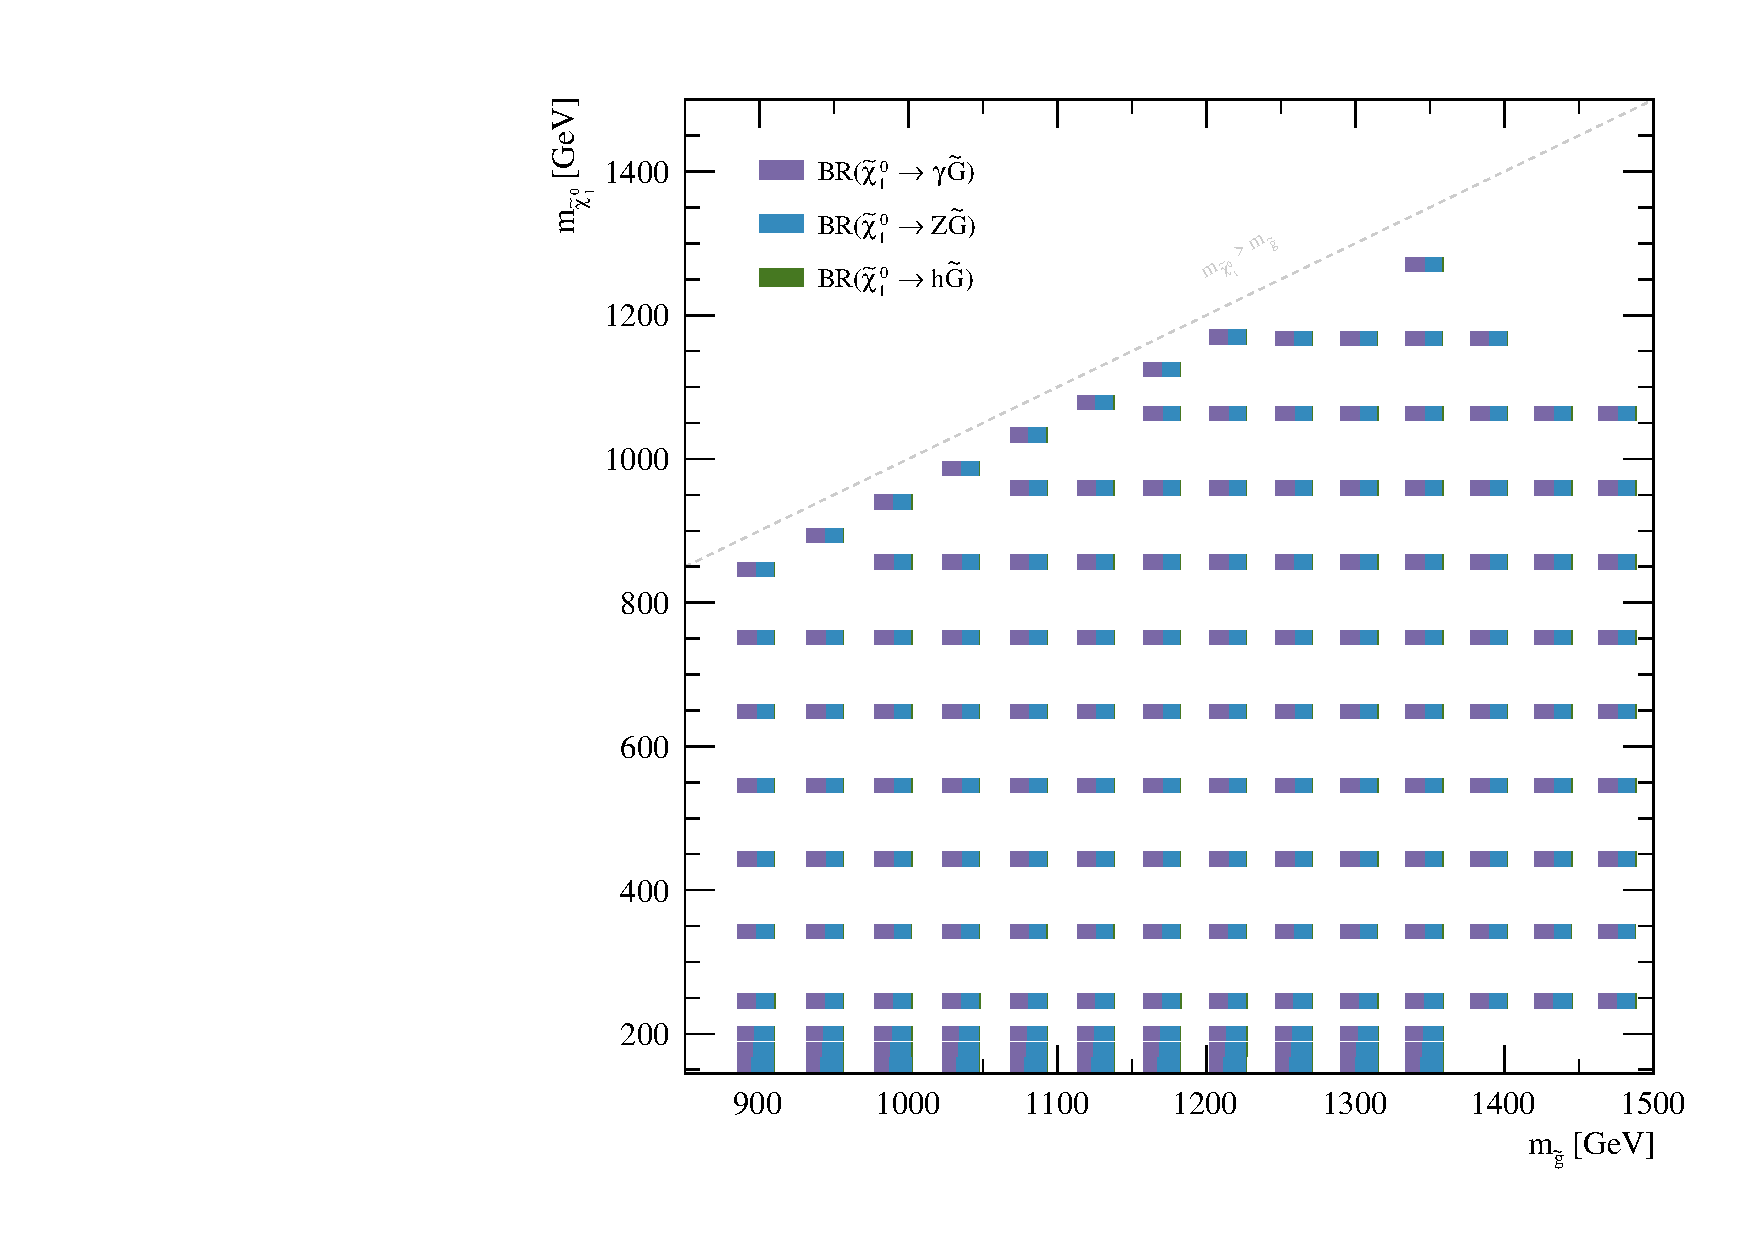
\includegraphics[width=0.6\textwidth]{figures/br_n1_X}

  \caption{Tasas de decaimiento (BR) de los neutralinos LSP en $\gamma\gravino$, $\gamma Z$ y
  $\gamma h$ para los distintos puntos de la \emph{grid} en el plano \mgmn.}
  \label{fig:signal_br_n1}
\end{figure}



\subsection{Sección eficaz de producción}
\label{sec:xs_calc}

En el caso de procesos de producción de pares de gluinos o squarks, de los cuales
existe el cálculo a NLL, la sección eficaz se toma a NLO en la constante de acoplamiento
fuerte, y se incluye la suma de la emisión de gluones soft con precisión NLL,
realizada utilizando {\nllfast}\cite{Kramer:2012bx,Beenakker:1996ch,Kulesza:2008jb,Kulesza:2009kq,Beenakker:2009ha,Beenakker:2011fu}.

En el caso de la producción de otro tipo de procesos, como la producción electrodébil de
partículas supersimétricas, se utilizan
las secciones eficaces calculadas a NLO usando {\prospino} \cite{Beenakker:1996ed}.


\newcommand{\pdfcteqpm}{\ensuremath{\Delta\mathrm{PDF}^{\pm}(\mathrm{CTEQ})}}
\newcommand{\scacteqpm}{\ensuremath{\Delta\mathrm{SCA}^{\pm}(\mathrm{CTEQ})}}

\newcommand{\pdfmstwpm}{\ensuremath{\Delta\mathrm{PDF}^{\pm}(\mathrm{MSTW})}}
\newcommand{\scamstwpm}{\ensuremath{\Delta\mathrm{SCA}^{\pm}(\mathrm{MSTW})}}

\newcommand{\alphap}{\ensuremath{\alpha_s_+}}
\newcommand{\alpham}{\ensuremath{\alpha_s^-}}
\newcommand{\alphapm}{\ensuremath{\alpha_s^{\pm}}}

Las incertezas debidas a la elección de la escala de renormalización y
factorización como también aquellas asociadas a la PDF, son obtenidas utilizando {\nllfast} o
calculadas con {\prospino}. A fin de combinar todas estas predicciones y obtener
una incerteza total, se siguen las recomendaciones PDF4LHC\cite{Botje:2011sn}.
Para esto se define la envolvente de las predicciones a la sección eficaz usando
el intervalo a 68\% CL del conjunto de PDFs CTEQ (incluyendo la incerteza en
$\alpha_s$) y MSTW, junto con las variaciones de las escalas. La sección eficaz
nominal se obtiene usando el punto medio de la envolvente y la incerteza como la
mitad del ancho de la misma. Matemáticamente si {\pdfcteqpm} y {\scacteqpm} son
las variaciones en $\pm 1\sigma$ de las PDF CTEQ,  {\pdfmstwpm} y {\scamstwpm}
son las variaciones en $\pm 1\sigma$ en la PDF MSTW, y {\alphapm} son las
correspondientes incertezas de la constante de acoplamiento fuerte, entonces,

\begin{align}
  \Delta\mathrm{CTEQ}^{\pm} &= \sqrt{(\pdfcteqpm)^2 + (\scacteqpm)^2 + (\alphapm)^2} \\
  \Delta\mathrm{MSTW}^{\pm} &= \sqrt{(\pdfmstwpm)^2 + (\scamstwpm)^2}
\end{align}

Los correspondientes extremos por arriba y abajo de la envolvente pueden calcularse a partir de estos:

\begin{align}
  U &= \max(\Delta\mathrm{CTEQ}^\mathrm{nom} + \Delta\mathrm{CTEQ}^{+},\quad \Delta\mathrm{MSTW}^\mathrm{nom} + \Delta\mathrm{MSTW}^{+}) \\
  L &= \min(\Delta\mathrm{CTEQ}^\mathrm{nom} - \Delta\mathrm{CTEQ}^{-},\quad \Delta\mathrm{MSTW}^\mathrm{nom} - \Delta\mathrm{MSTW}^{-})
\end{align}
%
y la sección eficaz final ($\sigma$) y su incerteza simétrica ($\Delta\sigma$) se obtiene como:

\begin{equation}
  \sigma = (U+L)/2,\quad \Delta\sigma = (U-L)/2
\end{equation}


En la \cref{tab:signal_xs_strong} puede verse la sección eficaz de producción de
pares de gluinos para los distintos puntos de la grid de señal generada. La
sección eficaz de producción electrodébil de neutralinos/charginos se encuentra en la
\cref{tab:signal_xs_ewk}. En la \cref{fig:signal_xs} también se encuentra
graficada la sección eficaz como función de la masa de las partículas
producidas, mientras que en la \cref{fig:signal_xs_total} se puede apreciar la
fracción en la producción electrodébil comparada con la producción total.

\begin{table}[!htb]
  \centering
  \caption{Sección eficaz a NLO+NLL para la producción de gluinos para los distintos
    puntos de la \emph{grid} de señal. La última columna es la incerteza teórica.}
  \begin{tabular}{cccc}
    \hline
    $M_3$ [\gev] & $m_{\gluino}$ [\gev] & $\sigma$(NLO+NLL) [fb] & Incerteza Total [$\%$]\tabularnewline
    \hline
    800  &  885.5  & 69.05 & 22.5  \\
    850  &  931.7  & 44.92 & 23.8  \\
    900  &  977.6  & 29.73 & 25.2  \\
    950  &  1023.1 & 19.83 & 26.5  \\
    1000 &  1068.3 & 13.41 & 27.7  \\
    1050 &  1113.3 & 9.10 & 29.0  \\
    1100 &  1157.9 & 6.28 & 30.4  \\
    1150 &  1202.3 & 4.32 & 32.0  \\
    1200 &  1246.4 & 3.01 & 33.7  \\
    1250 &  1290.3 & 2.10 & 35.2  \\
    1300 &  1333.9 & 1.48 & 36.7  \\
    1350 &  1377.3 & 1.05 & 38.2  \\
    1400 &  1420.5 & 0.74 & 39.8  \\
    1450 &  1463.4 & 0.53 & 41.5  \\
    \hline
  \end{tabular}
  \label{tab:signal_xs_strong}
\end{table}

\begin{table}[!htb]
  \centering
  \caption{Sección eficaz total a NLO para la producción electrodébil de neutralinos y charginos
    para los distintos puntos de la grid de señal. La última columna  es la incerteza
    teórica. Más detalles se encuentran en la \cref{sec:syst_signal}.}
  \begin{tabular}{cccc}
    \hline
    $\mu$ [\gev] & $m_{\ninoone}$ [\gev] & $\sigma$(NLO) [fb] & Incerteza total [$\%$]\tabularnewline
    \hline
    150   & & 2680 & 6.3  \\
    175   & & 1420 & 6.7  \\
    200   & & 840 & 6.9   \\
    250   & & 280 & 6.4     \\
    350   & & 50 & 7.0    \\
    450   & & 13 & 7.6    \\
    550   & & 4.1 & 8.0  \\
    650   & & 1.4 & 8.5   \\
    750   & & 0.53 & 8.9  \\
    850   & & 0.21 & 9.3  \\
    950   & & 0.0857 & 10.3  \\
    1050  & & 0.0356 & 11.0  \\
    1150  & & 0.0155 & 13.3   \\
    1250  & & 0.00667 & 16.9   \\
    \hline
  \end{tabular}
  \label{tab:signal_xs_ewk}
\end{table}


\begin{figure}[!htb]
  \centering
  \includegraphics[width=0.49\textwidth]{figures/SigXsec_strong}
  \includegraphics[width=0.49\textwidth]{figures/SigXsec_ewk}

  \caption{Sección eficaz de producción de pares de gluinos como función del parámetro $M_3$ (izquierda)
    y de pares de neutralinos/charginos como función del parámetro $\mu$ (derecha).}
  \label{fig:signal_xs}
\end{figure}

\begin{figure}[!htb]
  \centering
  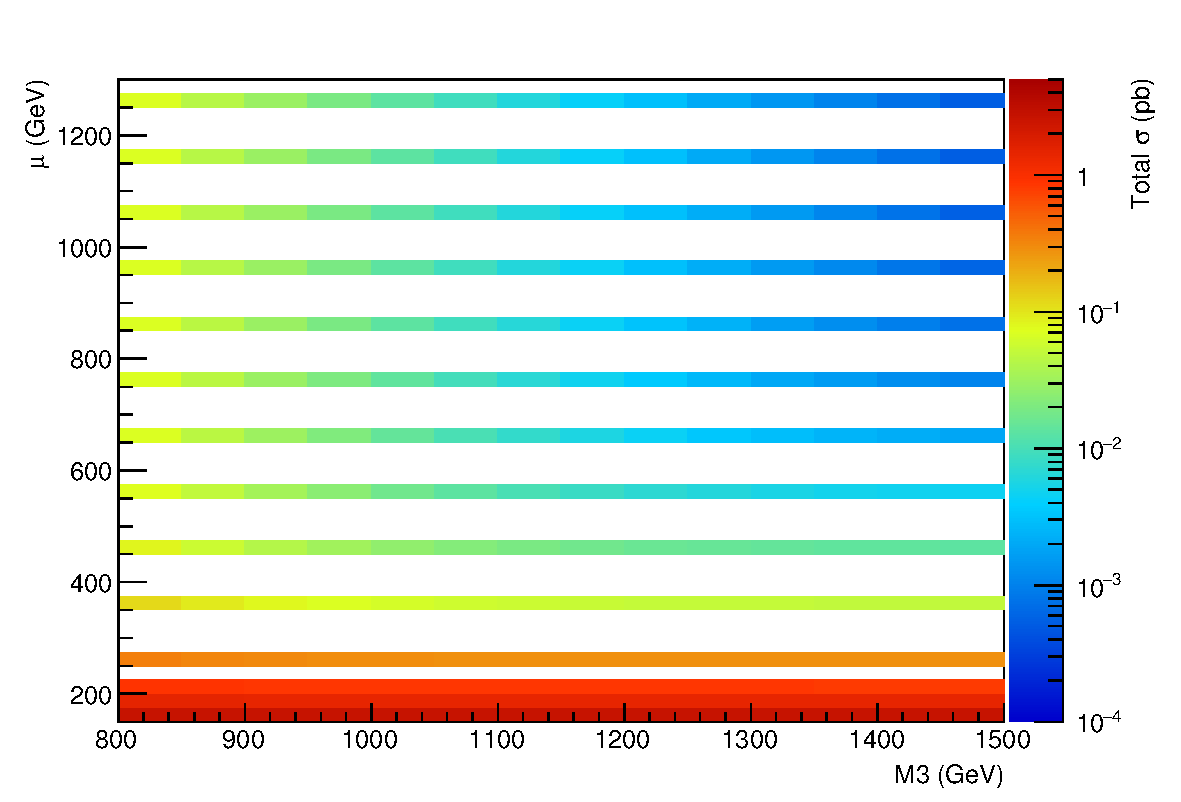
\includegraphics[width=0.49\textwidth]{figures/SigXsec_total}
  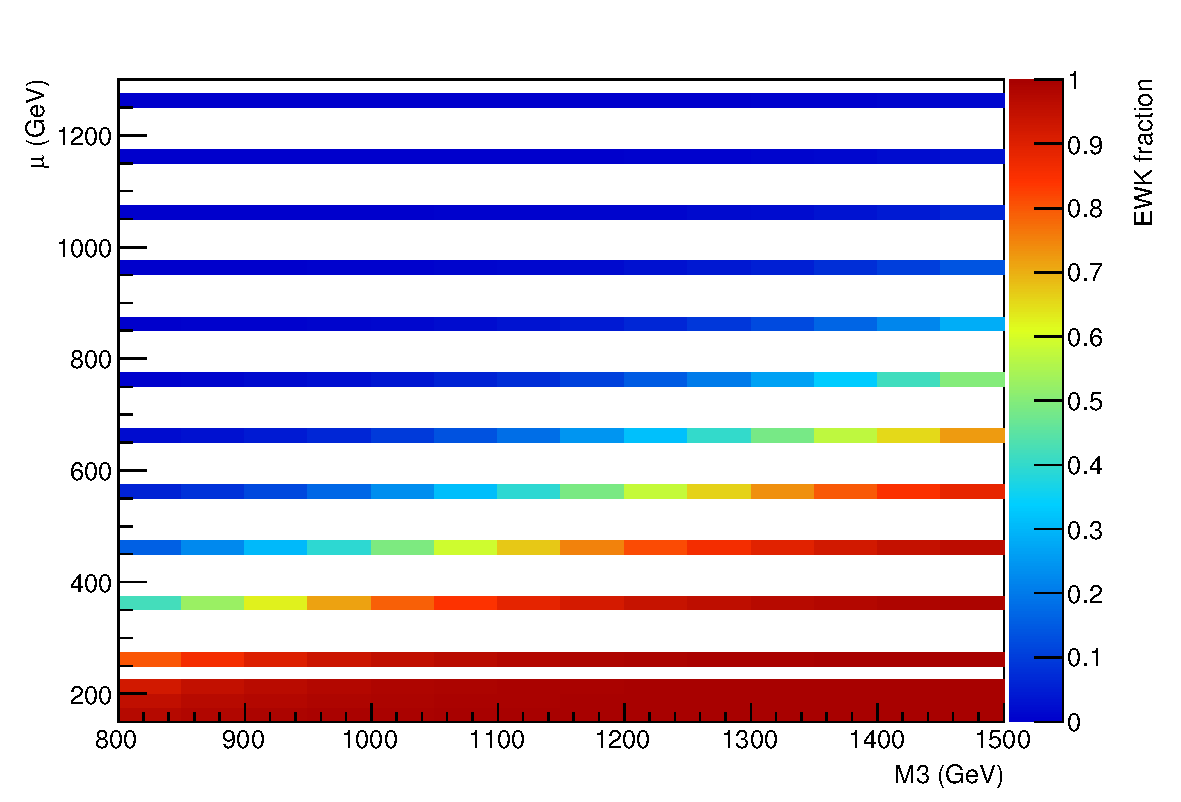
\includegraphics[width=0.49\textwidth]{figures/SigXsec_ewkFrac}
  \caption{Sección eficaz total (izquierda) y fracción relativa
    de producción electrodébil (derecha).}
  \label{fig:signal_xs_total}
\end{figure}
